%\setchapterimage{bandeau}
\chapter*{TD \arabic{cptTD} \\ 
Vision en réalité augmentée pour hélicoptère \ifnormal $\star$ \else \fi \iftdifficile $\star\star\star$ \else \fi -- 
\ifprof Corrigé \else Sujet \fi}
\addcontentsline{toc}{section}{TD \arabic{cptTD} :
Vision en réalité augmentée pour hélicoptère \ifnormal $\star$ \else \fi \iftdifficile $\star\star\star$ \else \fi -- 
\ifprof Corrigé \else Sujet \fi}

\iflivret \stepcounter{cptTD} \else
\ifprof  \stepcounter{cptTD} \else \fi
\fi

\setcounter{question}{0}
\marginnote{Concours Centrale Supelec 2014.}
\marginnote[1cm]{
\UPSTIcompetence[2]{C1-02}
\UPSTIcompetence[2]{C2-04}}

\begin{marginfigure}[3.5cm]
\centering
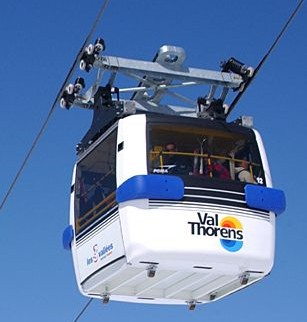
\includegraphics[width=\linewidth]{fig_00}
\end{marginfigure}


\section*{Mise en situation}
Le FLIR est une boule optronique modulaire pouvant intégrer plusieurs capteurs différents dont une caméra
thermique, une caméra couleur TV HD, ainsi qu’une caméra très bas niveau de lumière. Cet ensemble est
orientable et gyrostabilisé, c’est-à-dire en particulier que les caméras sont capables de garder une même ligne
de visée par rapport au référentiel terrestre, quels que soient les mouvements de l’hélicoptère NH90 qui sera
appelé porteur dans la suite du sujet.


\begin{marginfigure}[4cm]
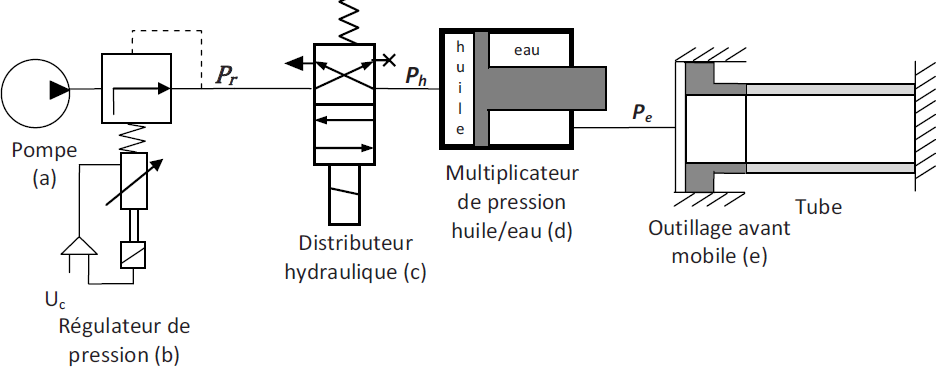
\includegraphics[width=\linewidth]{fig_01}
%\textit{}
\end{marginfigure}

Afin de limiter l’influence des vibrations du porteur sur la ligne de visée et augmenter la précision de son orientation,
les ingénieurs ont choisi de décomposer l’axe motorisé d’élévation en deux étages.
Le premier étage, appelé étage gros d’élévation ($ge$), est en prise directe avec l’air et est donc soumis aux effets
aérodynamiques lors des mouvements du porteur. L’étage gros d’élévation est lui même en liaison pivot, d’axe $\axe{P}{y_e}$, avec l’axe motorisé d’azimut. Le second, appelé étage fin d’élévation ($fe$), est protégé des effets aérodynamiques grâce au carter sphérique solidaire de l’étage gros. Cet étage est en liaison pivot,
d’axe $\axe{P}{y_e}$, avec l’étage gros d’élévation. L’inertie des éléments déplacés par l’étage fin d’élévation est plus faible
que celle de l’étage gros d’élévation et les choix de guidage et de motorisation permettent d’atteindre des accélérations
et des vitesses élevées. Cependant, l’amplitude du mouvement de l’étage fin est limitée. 



Les performances de l’étage fin d’élévation sont données dans le tableau ci-contre. 
\begin{margintable}
\begin{tabular}{p{3cm}l}
\hline
\textbf{Exigence} & Valeur \\ \hline
Temps de réponse à 5\% & <\SI{40}{ms} \\ 
Écart statique & nul \\ 
Marge de phase & $\Delta \phi = 60\degres$ \\ \hline
\end{tabular}
\end{margintable}

La consigne de vitesse $\dot{\theta}_{\text{fe0 cons}}(t)= \omega_{\text{fe0 cons}}(t)$ est établie par rapport au référentiel galiléen $\rep{0}$. Elle est calculée à partir de la détection de posture  de la tête du pilote et des informations 
d’orientation du porteur par rapport au référentiel terrestre $\rep{0}$ obtenues par la centrale inertielle du porteur.


\marginnote{
$k_{\text{cfe}}=\SI{10,2}{N.A^{-1}}$, $k_{\text{vfe}}=\SI{10,2}{V.s.m^{-1}}$, on note 
$K_{\text{fe}}=k_{\text{cfe}}=k_{\text{vfe}}$, $R_{\text{fe}}=\SI{7,5}{\Omega}$. }
\begin{center}
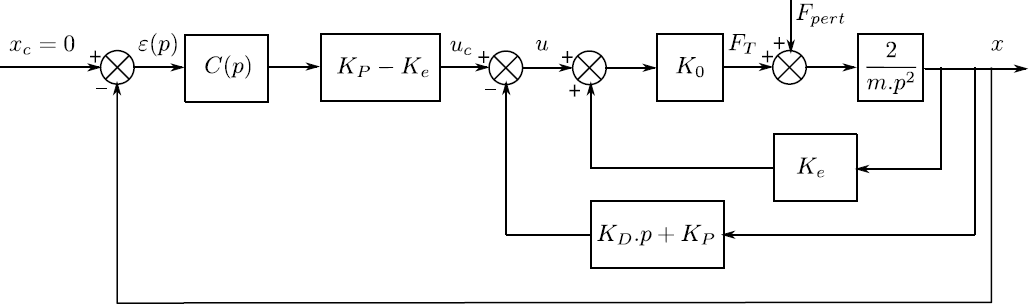
\includegraphics[width=.8\linewidth]{fig_02}
%\textit{}

\end{center}

Dans un premier temps, l’asservissement de vitesse n’est pas corrigé, c’est-à-dire que $H_{\text{cor }fe}(p)=1$.


\question{Exprimer littéralement et sous forme canonique la fonction de transfert $H_{fe1}(p)=\dfrac{\Omega_{fe0}(p)}{\Omega_{fe0\text{ cons}}(p)}$, en fonction de $K_1$, $\tau_{\text{gyro}}$, $M_{\text{eq}}$, $K_{fe}$ et $R_{fe}$.}

\ifprof
\begin{corrige}
\end{corrige}
\else
\fi
Compte tenu des temps de réponse à observer, on montre que $H_{fe1}(p$ peut se mettre sous la forme simplifiée suivante : $H_{fe1}(p)=\dfrac{0,5}{1+3,65\times 10^{-1}p+6\times 10^{-4}p^2}$.
\question{En utilisant l’abaque de la figure suivante, déterminer le temps de réponse à 5\% et l’écart statique de l’asservissement en vitesse de l’étage fin d’élévation en réponse à un échelon de vitesse unitaire. Conclure sur le
respect des performances en rapidité et en précision.}
\ifprof
\begin{corrige}
\end{corrige}
\else
\fi


\begin{marginfigure}
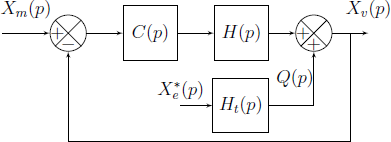
\includegraphics[width=\linewidth]{fig_03}
%\textit{}
\end{marginfigure}


On propose d’utiliser un correcteur proportionnel intégral de la forme $H_{\text{cor }fe}(p)=K_{\text{\text{pfe}}}\left(1+\dfrac{1}{T_{\text{ife}}p}\right)$. La fonction de transfert en boucle ouverte de l’asservissement en vitesse de l’étage fin d’élévation devient alors 
$
H_{\text{BOfe}}(p)=K_{\text{pfe}}\left( 1+\dfrac{1}{T_{\text{ife}}p}\right) \dfrac{1}{1+0,75p} \dfrac{1}{1+1,6\times 10^{-3}p}
$.

La figure suivante correspond aux tracés des diagrammes de Bode réels de $H_{\text{BOfe}}(j\omega)$ 
pour $K_{\text{pfe}}=1$ et $T_{\text{ife}}=\SI{0,1}{s}$ puis $T_{\text{ife}}=\SI{0,01}{s}$.


\begin{marginfigure}
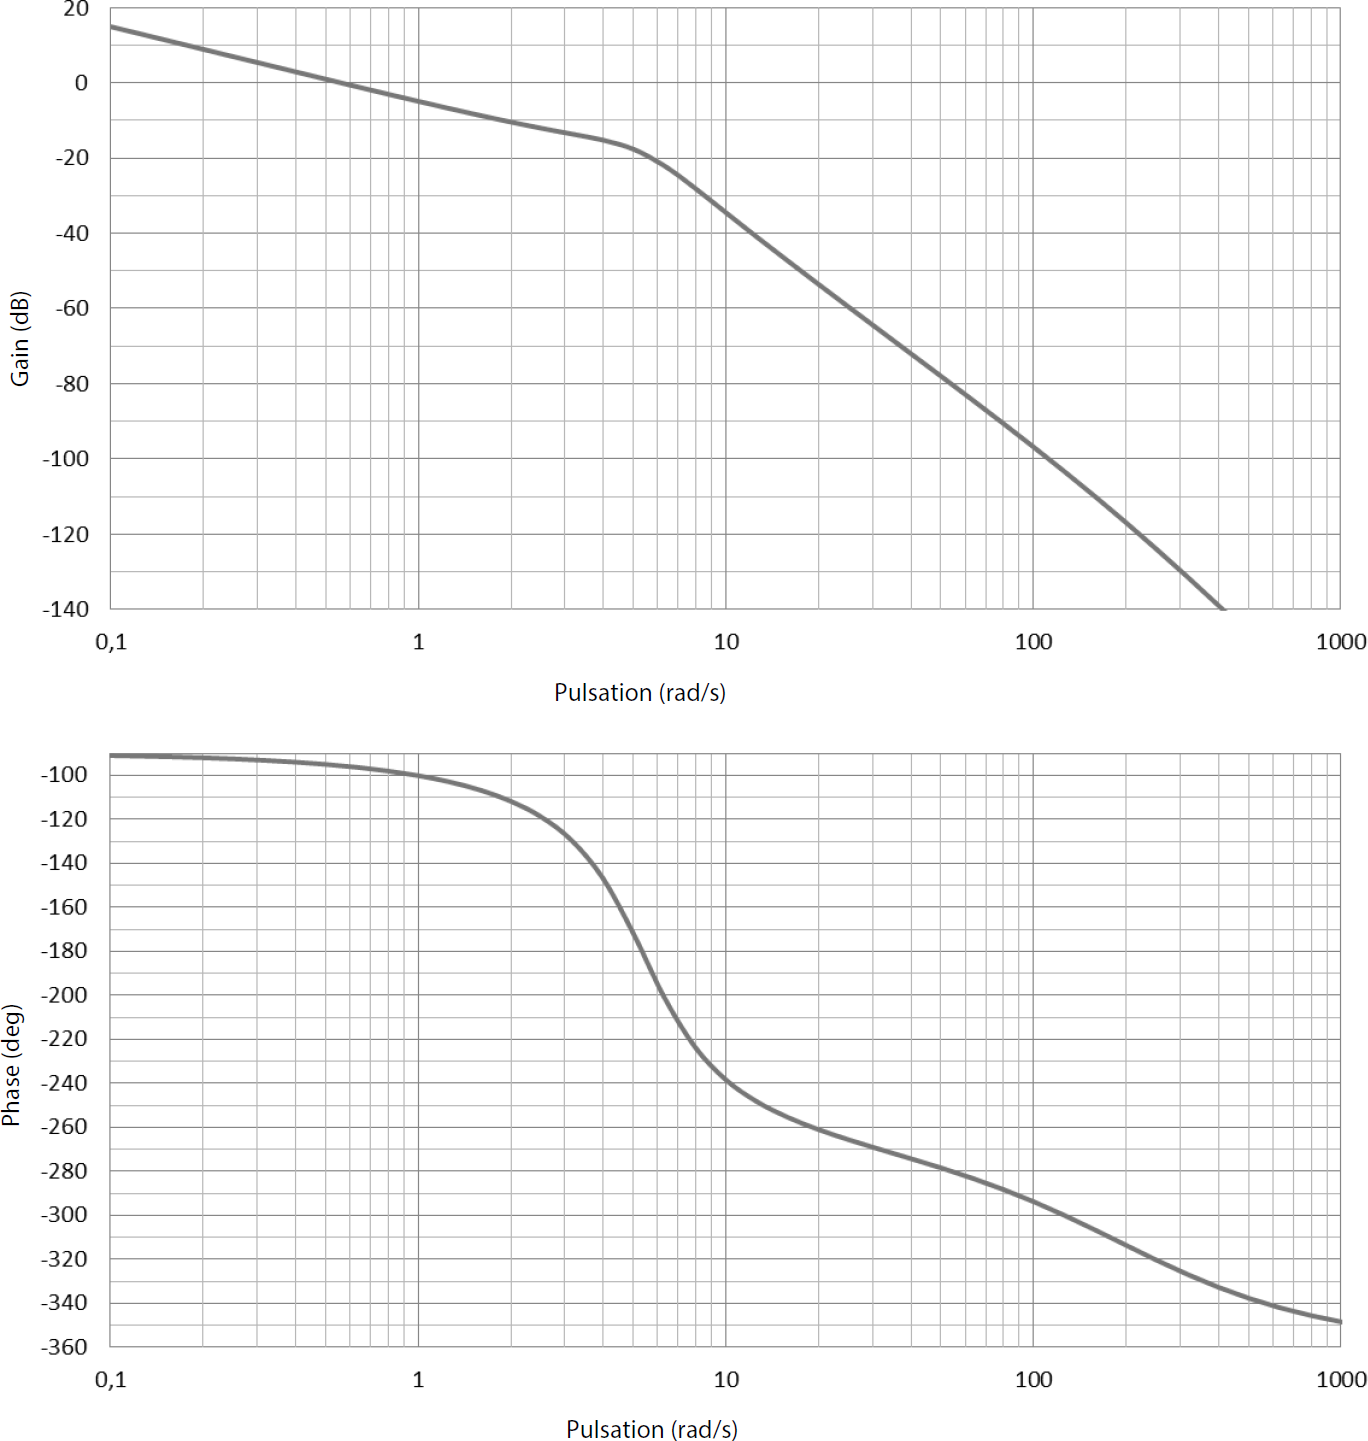
\includegraphics[width=\linewidth]{fig_04}
%\textit{}
\end{marginfigure}


\question{Sur cette même figure, tracer le diagramme de phase asymptotique de $H_{\text{BOfe}}(j\omega)$
(Bode) pour $T_{\text{ife}}=\SI{0,1}{s}$, en indiquant la pulsation $\dfrac{1}{T_{\text{ife}}}$.}
\ifprof
\begin{corrige}
\end{corrige}
\else
\fi

La lecture du tracé réel de la phase met en évidence un maximum à la pulsation $\omega_{\text{max}}$ telle que $\omega_{\text{max}}\in \left[\dfrac{1}{T_{\text{ife}}};600 \right]\text{rad s}^{-1}$.

\question{En supposant que le tracé réel semi-logarithmique de la phase est symétrique autour de $\omega_{\text{max}}$, calculer la valeur de $T_{\text{ife}}$ comprise dans la décade $\left[\SI{0,01}{s}; \SI{0,1}{s}\right]$ qui permet de régler ce maximum à \SI{-120}{\degres}.}
\ifprof
\begin{corrige}
\end{corrige}
\else
\fi

\question{Pour le réglage de $T_{\text{ife}}$ calculé à la question précédente avec $K_{\text{pfe}}= 1$ et à partir des tracés réels du document réponse, calculer la valeur de $K_{\text{pfe}}$ qui permet de respecter le critère de marge de phase.}
\ifprof
\begin{corrige}
\end{corrige}
\else
\fi


Le modèle est complété en utilisant les réglages déterminés aux deux questions précédentes pour $K_{\text{pfe}}$ et $T_{\text{ife}}$. Afin de
prendre en compte les caractéristiques du moteur linéaire, une saturation d’alimentation du moteur à \SI{24}{V} est
ajoutée ainsi qu’une modification de la commande associée qui n’est pas étudiée ici et qui ne modifie pas les
réglages de $K_{\text{pfe}}$ et $T_{\text{ife}}$ déterminés précédemment. La réponse simulée $\omega_{fe0}(p)$ de l’étage fin d’élévation à une
consigne de vitesse en échelon $\omega_{fe0 \text{ cons}}(t) = \SI{1}{rad.s^{-1}}$ est donnée sur la figure suivante.

\begin{center}
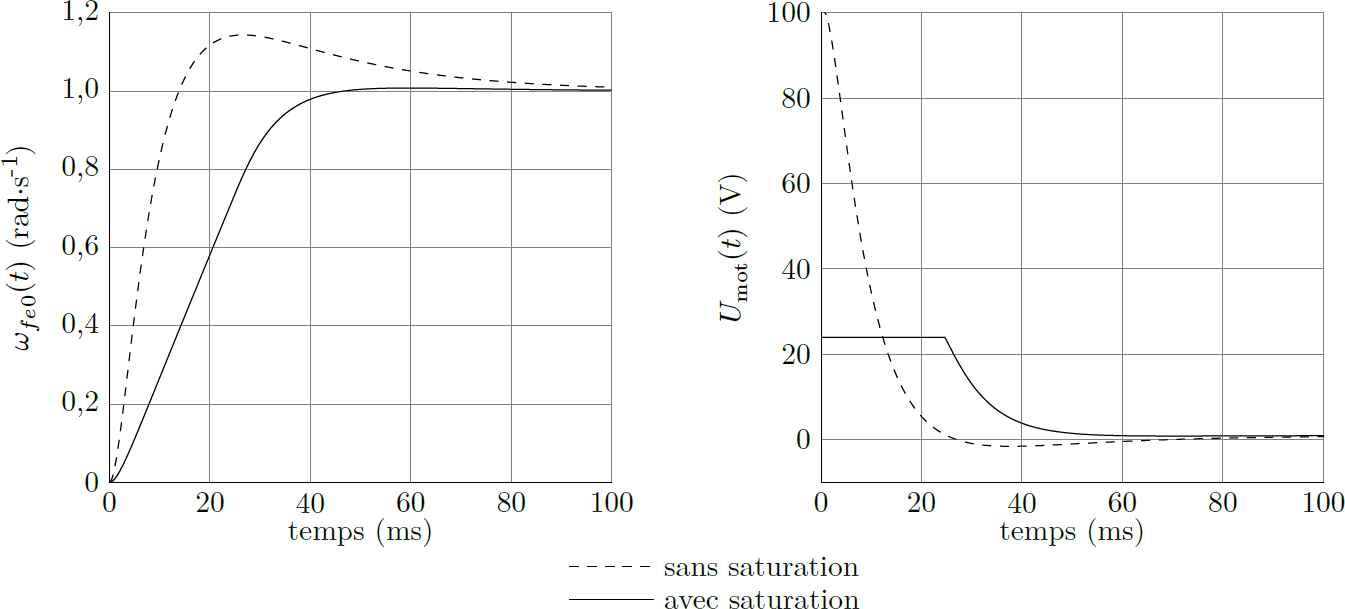
\includegraphics[width=.8\linewidth]{fig_05_a}
%\textit{}
\end{center}




\question{D’après la figure précédente, définir le temps pendant lequel la tension du moteur linéaire a été saturée et expliquer les effets de cette saturation sur les performances simulées par rapport aux performances simulées
en gardant le modèle linéaire. Conclure sur la pertinence de la prise en compte de la saturation et sur les
performances de l’étage fin d’élévation.}
\ifprof
\begin{corrige}
\end{corrige}
\else
\fi

\subsection*{Synthèse : validation des performances simulées du FLIR}
\begin{obj}
Simuler le comportement de l’axe motorisé d’élévation du FLIR et vérifier s’il respecte le cahier des
charges.
\end{obj}



À l’instar de l’étage fin d’élévation, l’étage gros d’élévation est également asservi, mais en position angulaire. Il
doit permettre à l’étage fin d’élévation de vérifier l’hypothèse émise précédemment, soit $\vect{u}\simeq \vect{z_e}$, c’est-à-dire que l’angle $\beta(t)$ doit rester dans l’intervalle $[-5\degres, +5\degres]$.
Un capteur LVDT (Linear Variable Differential Transformer) permet de mesurer l’écart entre l’orientation de
l’étage fin d’élévation et l’étage gros d’élévation $\beta(t)=\theta_{fe0}(t)-\theta_{ge0}(t)$. Le modèle d’asservissement de l’axe
motorisé d’élévation est alors celui donné sur la figure suivante. 

\begin{center}
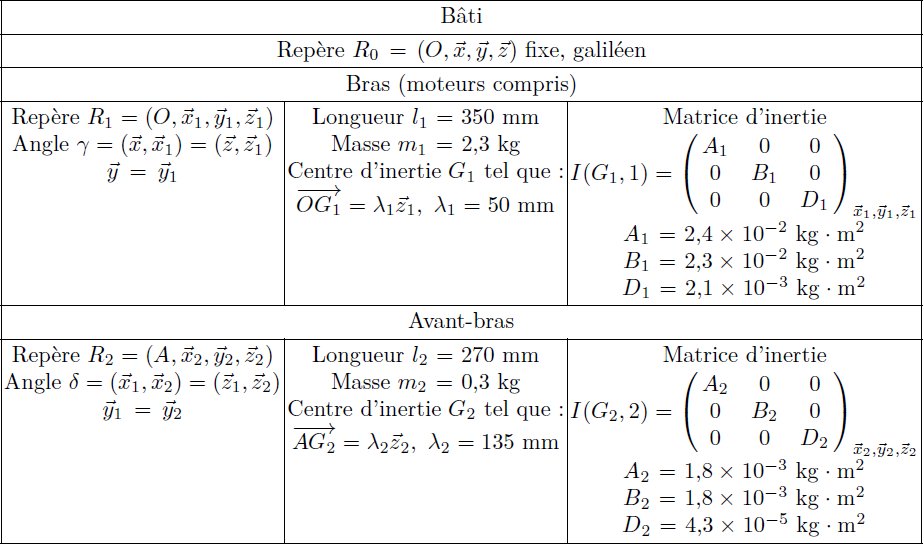
\includegraphics[width=.8\linewidth]{fig_06}
%\textit{}
\end{center}


\begin{marginfigure}
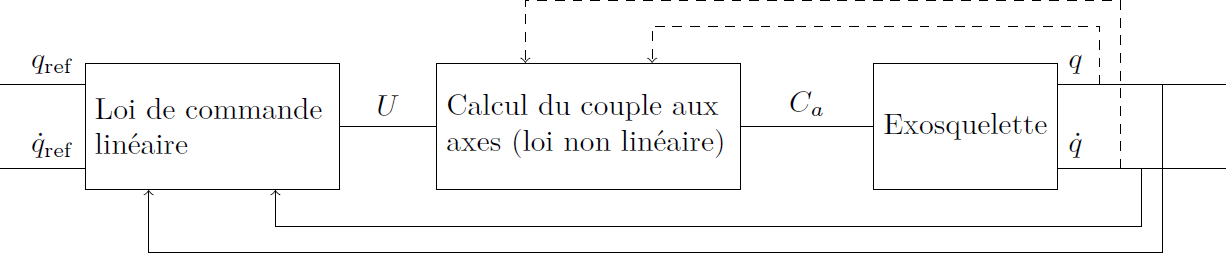
\includegraphics[width=\linewidth]{fig_07}
%\textit{}
\end{marginfigure}

La figure ci-contre correspond à une mesure expérimentale du taux de rotation de la tête d’un pilote pour un mouvement
d’élévation de sa ligne de visée. Ce signal peut alors être utilisé comme signal de consigne envoyé à l’axe motorisé
d’élévation du FLIR.





Pour simuler le modèle de l’axe motorisé d’élévation et comparer ses performances au cahier des charges, il est nécessaire de définir un signal de consigne  $\omega_{fe0 \text{ cons}}(t)$ composé des signaux canoniques utilisés
en automatique.

\question{À partir de la figure précédente et en utilisant les signaux échelon et/ou rampe, proposer un modèle temporel
associé au signal de consigne $\omega_{fe0 \text{ cons}}(t)$ exprimé en $\text{rad\, s}^{-1}$, sous la forme d’un tracé simple en fonction du temps en seconde. Tracer l’allure de $\theta_{fe0 \text{ cons}}(t)$, exprimé en rad, qui correspond à l’évolution temporelle de la ligne de visée du pilote dans ce cas. Préciser les valeurs des points caractéristiques de ces deux courbes.}
\ifprof
\begin{corrige}
\end{corrige}
\else
\fi

\question{À partir des deux tracés précédents, indiquer quels critères du cahier des charges peuvent être validés en utilisant ce signal de consigne dans la simulation du comportement de l’axe motorisé d’élévation
du FLIR.}
\ifprof
\begin{corrige}
\end{corrige}
\else
\fi

Après avoir dimensionné et implanté le correcteur proportionnel intégral (noté PI) au sein du modèle de l’étage
gros d’élévation, on simule l’évolution de $\beta(t)= \theta_{fe0}(t) -\theta_{ge0}(t)$ pour le signal de consigne $\omega_{fe0 \text{ cons}}(t)$
établi à partir de la mesure de la figure précédente. Les résultats de simulation sont donnés sur les figures suivantes.

\question{À partir des figures suivantes:
\begin{itemize}
\item vérifier si l’hypothèse $\vect{u}\simeq \vect{z_e}$ reste valide ;
\item pour chaque critère du cahier des charges à l’aide de tracés sur les figures,
conclure sur l’aptitude du FLIR à respecter les performances du cahier des charges en comparant les valeurs
numériques mesurées sur les résultats de simulation à celles du cahier des charges.
\end{itemize}}
\ifprof
\begin{corrige}
\end{corrige}
\else
\fi
\ifprof
\else
\footnotesize


\begin{table*}[!h]
\centering
\begin{tabular}{cccc}
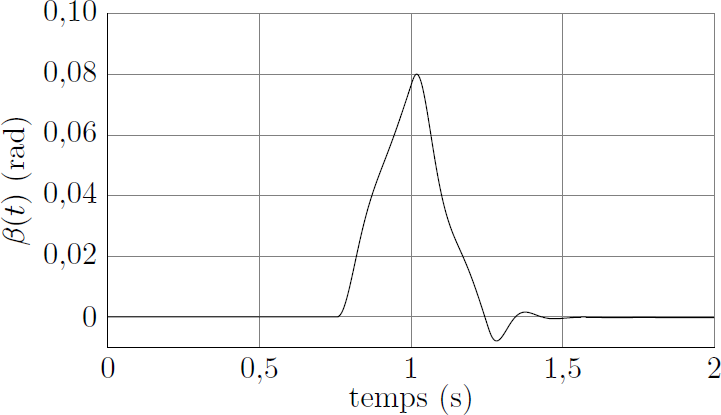
\includegraphics[width=.22\linewidth]{fig_08_a} & 
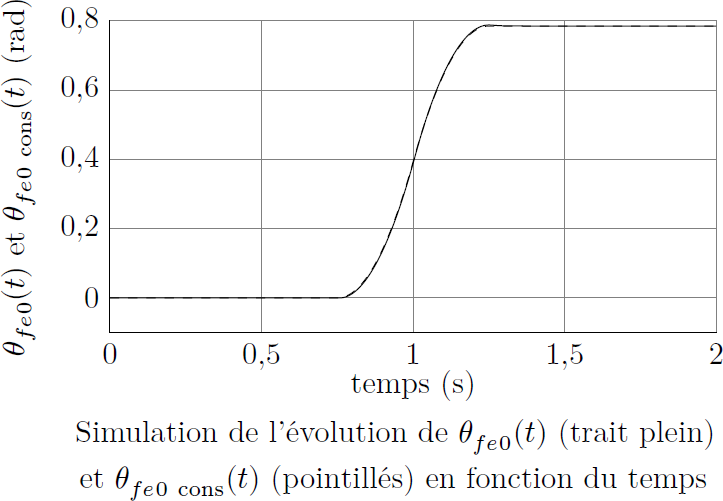
\includegraphics[width=.22\linewidth]{fig_08_b} &
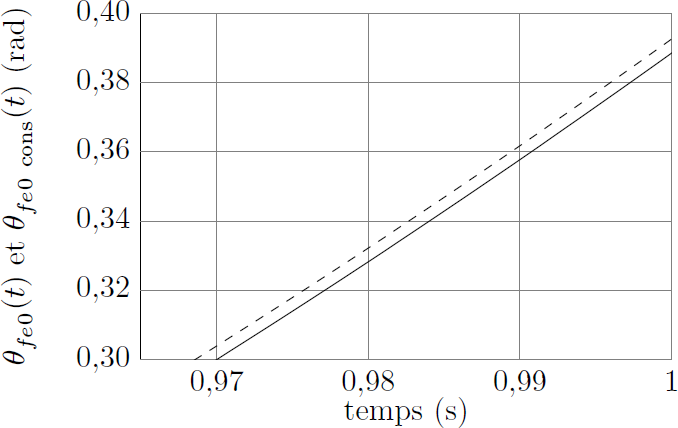
\includegraphics[width=.22\linewidth]{fig_08_c} &
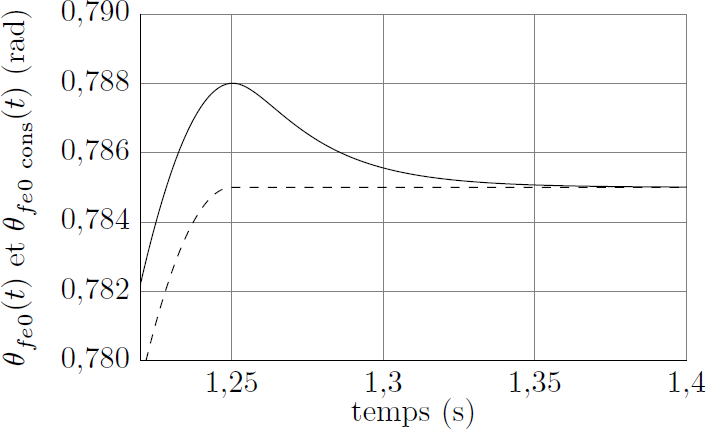
\includegraphics[width=.22\linewidth]{fig_08_d}
\end{tabular}
\caption{Zooms de $\theta_{fe0}(t)$ (trait plein) et $\theta_{fe0\text{ cons}}(t)$ (pointillés) \\ en fonction de temps}
\end{table*}

%\begin{marginfigure}
%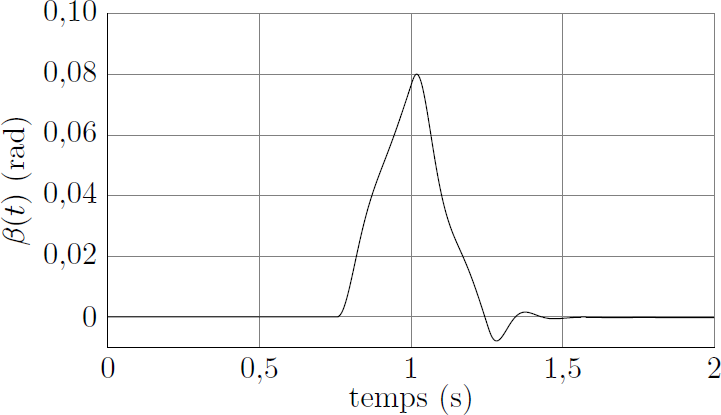
\includegraphics[width=\linewidth]{fig_08_a}
%\textit{}
%\end{marginfigure}
%
%\begin{marginfigure}
%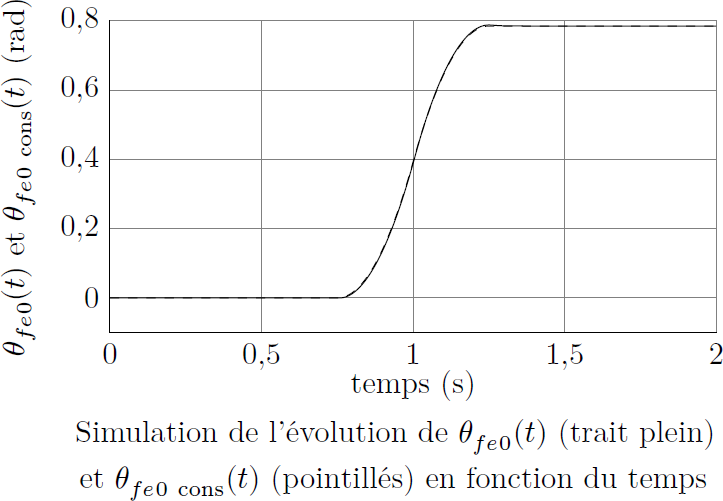
\includegraphics[width=\linewidth]{fig_08_b}
%\textit{}
%\end{marginfigure}
%
%\begin{marginfigure}
%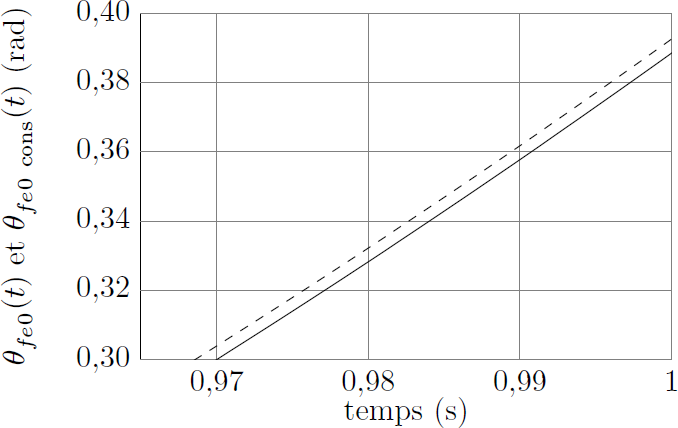
\includegraphics[width=\linewidth]{fig_08_c}
%\textit{}
%\end{marginfigure}
%
%\begin{marginfigure}
%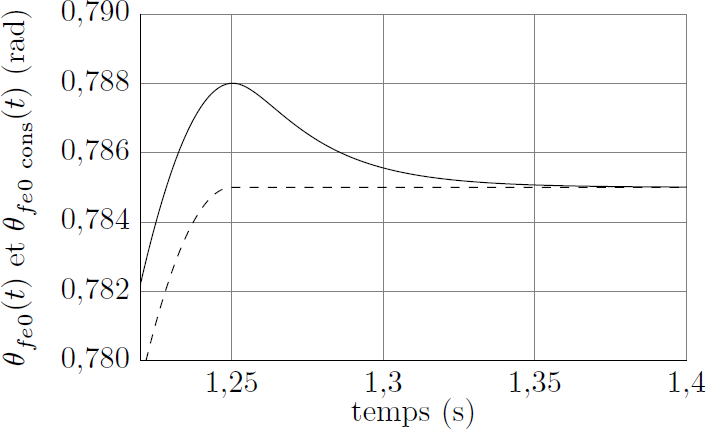
\includegraphics[width=\linewidth]{fig_08_d}
%\caption{Zooms de $\theta_{fe0}(t)$ (trait plein) et $\theta_{fe0\text{ cons}}(t)$ (pointillés) \\ en fonction de temps}
%\end{marginfigure}


%\begin{enumerate}
%\item 
%
%\item 
%\end{enumerate}
\normalsize
\fi

